\chapter{設計}
\label{chap:design}

本章では次世代のARナビゲーションシステム「HypAR Touch」の要件と設計について述べる

\newpage

\section{要件}
前章で整理したARナビゲーションシステムの問題点を踏まえた上でHypAR Touchシステムの要件を整理する。
\begin{itemize}
  \item 手軽になインタラクションでアプリケーションの起動と位置キャリブレーションができる
  \item 個別にコンテキストを簡単に指定できるようにし、汎用性をもたせる
  \item ARでの表示情報を容易に登録・編集できる
  \item ハイパーリンクを利用し関連情報を参照・管理することができる
\end{itemize}
これらの要件を満たすARナビゲーションシステムは、NFCをタッチするインタラクションとハイパーテキストの編集環境であるWikiを組み合わせによって実現できる。

\section{HypAR Touch}
本研究で提案するARナビゲーションシステムであるHypAR Touchの基本構成と使い方を解説する。

\subsection{基本構成}
本研究で提案するARナビゲーションシステムHypAR Touchはモバイル端末向けアプリケーションであるHypAR Touch アプリと専用のNFCタグ、WikiであるScrapboxで構成されている。

\paragraph*{HypAR Touchアプリ} 
HypAR TouchアプリはARでのナビゲーションを表示するモバイル端末向けネイティブアプリケーションである。
後述する専用のNFCタグにタッチすることでARナビゲーションを表示することができる。
NFC読み取り機能を持つAndroid\footnote{\textsf{TODO:todo}}端末とiOS\footnote{\textsf{TODO:todo}}端末に対応しており、現在流通する多くのモバイル端末で利用可能である。

\paragraph*{NFCタグ}
本システムではモバイル端末の位置情報検出および提示するナビゲーションの出し分けのためにNFCタグを利用している。
NFCタグにはISO/IEC 14443のTypeA\footnote{\textsf{TODO:todo}}に該当するNFCタグを利用しており、NDEF\footnote{\textsf{TODO:todo}}形式で情報を記録している。
このタグタイプと情報形式はNFC機能を持つほとんどのモバイル端末で読み取りがサポートされており、アプリを起動していない状態でのバックグラウンド読み取りに対応している。
さらにタグ内に記録する情報としてCustomURLSchemeを利用することでアプリが起動していない状態でもモバイル端末でNFCにタッチすることでHypAR Touchアプリを起動することが可能となる。

\paragraph*{Scrapbox}
Scrapbox(図\ref{fig:scrapbox})はGyazz\cite{Gyazz}をベースにして開発された、Nota\footnote{\textsf{https://www.notainc.com/ja}}社が運営しているWikiである。
本システムではScrapboxをARで表示する情報の登録・編集ツールとして利用している。
これはScrapboxが他のシステムには存在しない以下のようなHypAR Touchに適した特徴を持つためである。
\begin{itemize}
  \item シンプルで柔軟な記法をもつWYSIWYGエディタ
  
  入力/改行/段落/箇条書きといった基本的なテキスト編集を見たまま行える。
  
  \item 場所指定に最適なLocation記法
  
  Google MapsのURLを貼り付けるだけで地図を埋め込めるLocation記法\footnote{\textsf{https://scrapbox.io/help-jp/Location記法}}と呼ばれる機能があり地理情報を記述するのに適している。
  本システムではLocation記法でAR情報を表示する場所を指定している。

  \item シンプルなリンク記法によるハイパーリンクと関連ページリスト
  
  Scrapboxでは単語を\texttt{[]}で囲うだけで同一wiki内ページへのリンクとすることが可能である。
  さらにScrapboxページの下部には
  \begin{itemize}
      \item 別ページへのリンク
      \item 別ページからのリンク
      \item リンク先ページがリンクしているページ
  \end{itemize}
  といった関連ページリスト(図\ref{fig:scrapbox_related})が表示され、どのような情報と関連するのか一目瞭然に分かる。

\end{itemize}

\begin{figure}[h]
  \centering
  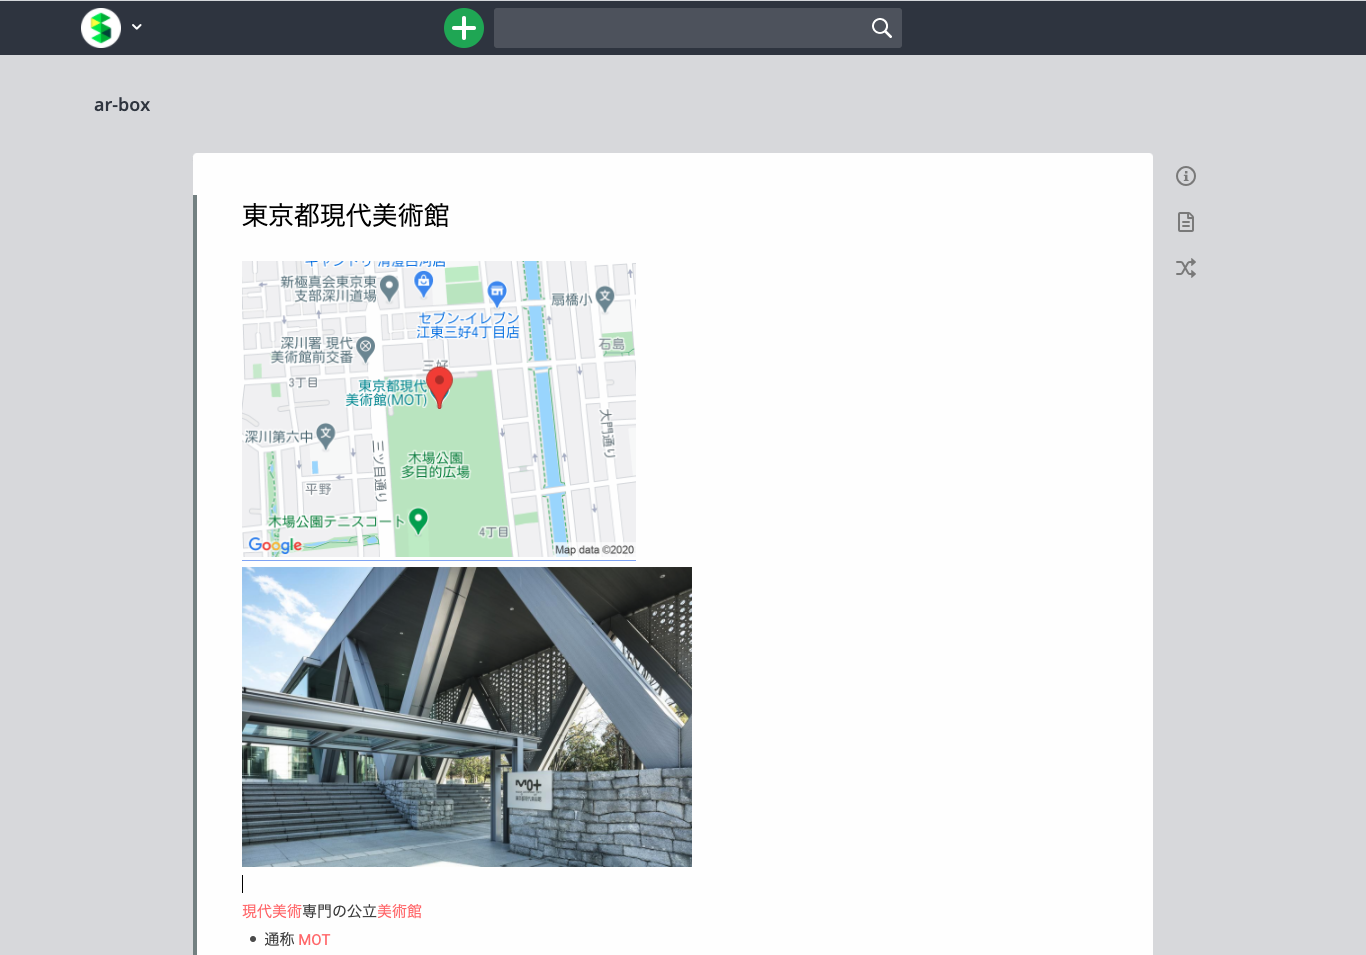
\includegraphics[width=100mm]{images/scrapbox_screen.png}
  \caption{Scrapboxの画面} \label{fig:scrapbox}
\end{figure}

\begin{figure}[h]
  \centering
  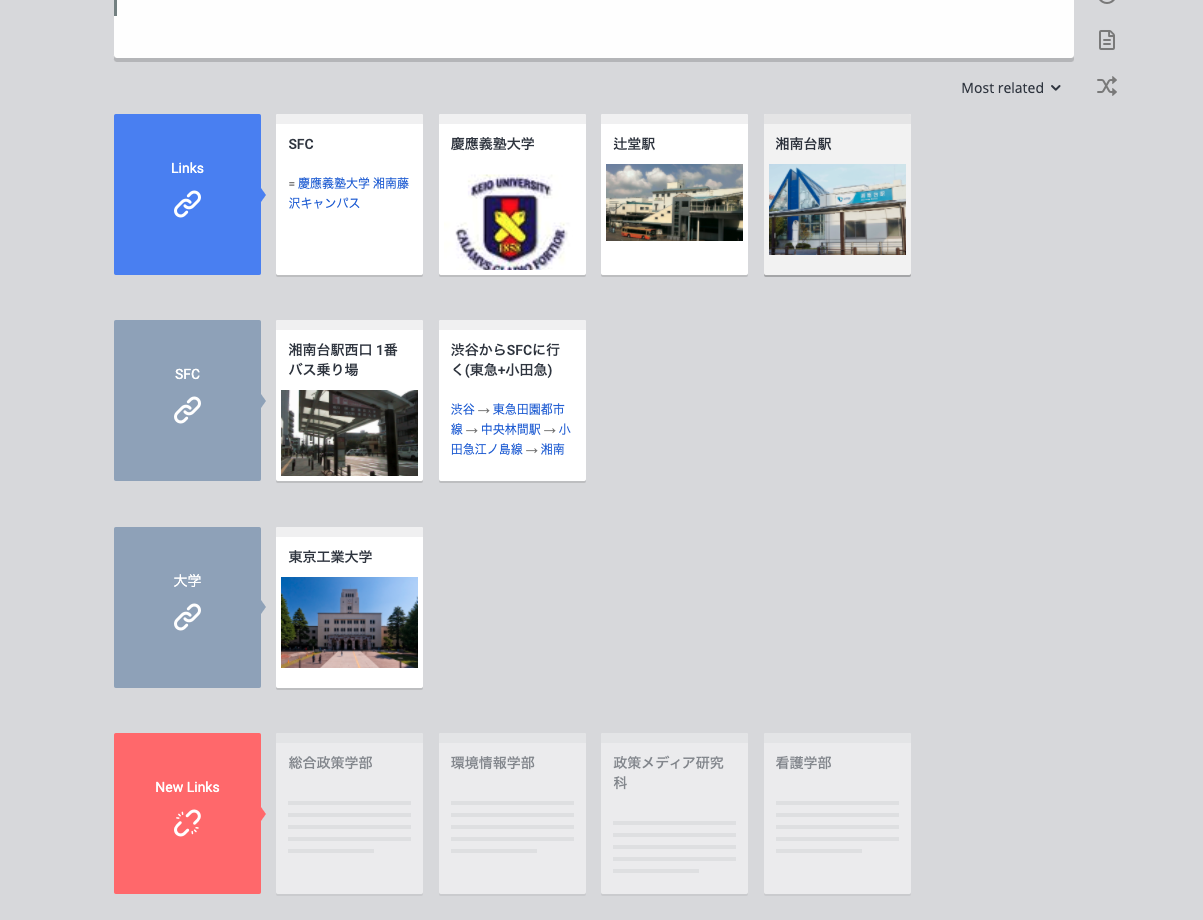
\includegraphics[width=100mm]{images/scrapbox_related_screen.png}
  \caption{Scrapboxの関連ページリスト} \label{fig:scrapbox_related}
\end{figure}

\subsection{使い方}

\subsubsection{HypAR Touchアプリによるナビゲーション閲覧}
\paragraph*{NFCタグにタッチする}
本アプリケーションは図\ref{fig:touch_nfc}のように専用の情報が書かれたNFCタグにタッチすることで起動し、ナビゲーションを開始する。
NFCにタッチすることで位置と向きを認識し、図\ref{fig:hypar_touch_init_screen}のように登録された情報をARで正しい位置に表示することができる。
また画面下部にあるスライダー(図\ref{fig:hypar_touch_slider})を右に動かすことでより遠くにある情報がARで見れるようになる。

\begin{figure}[h]
  \centering
  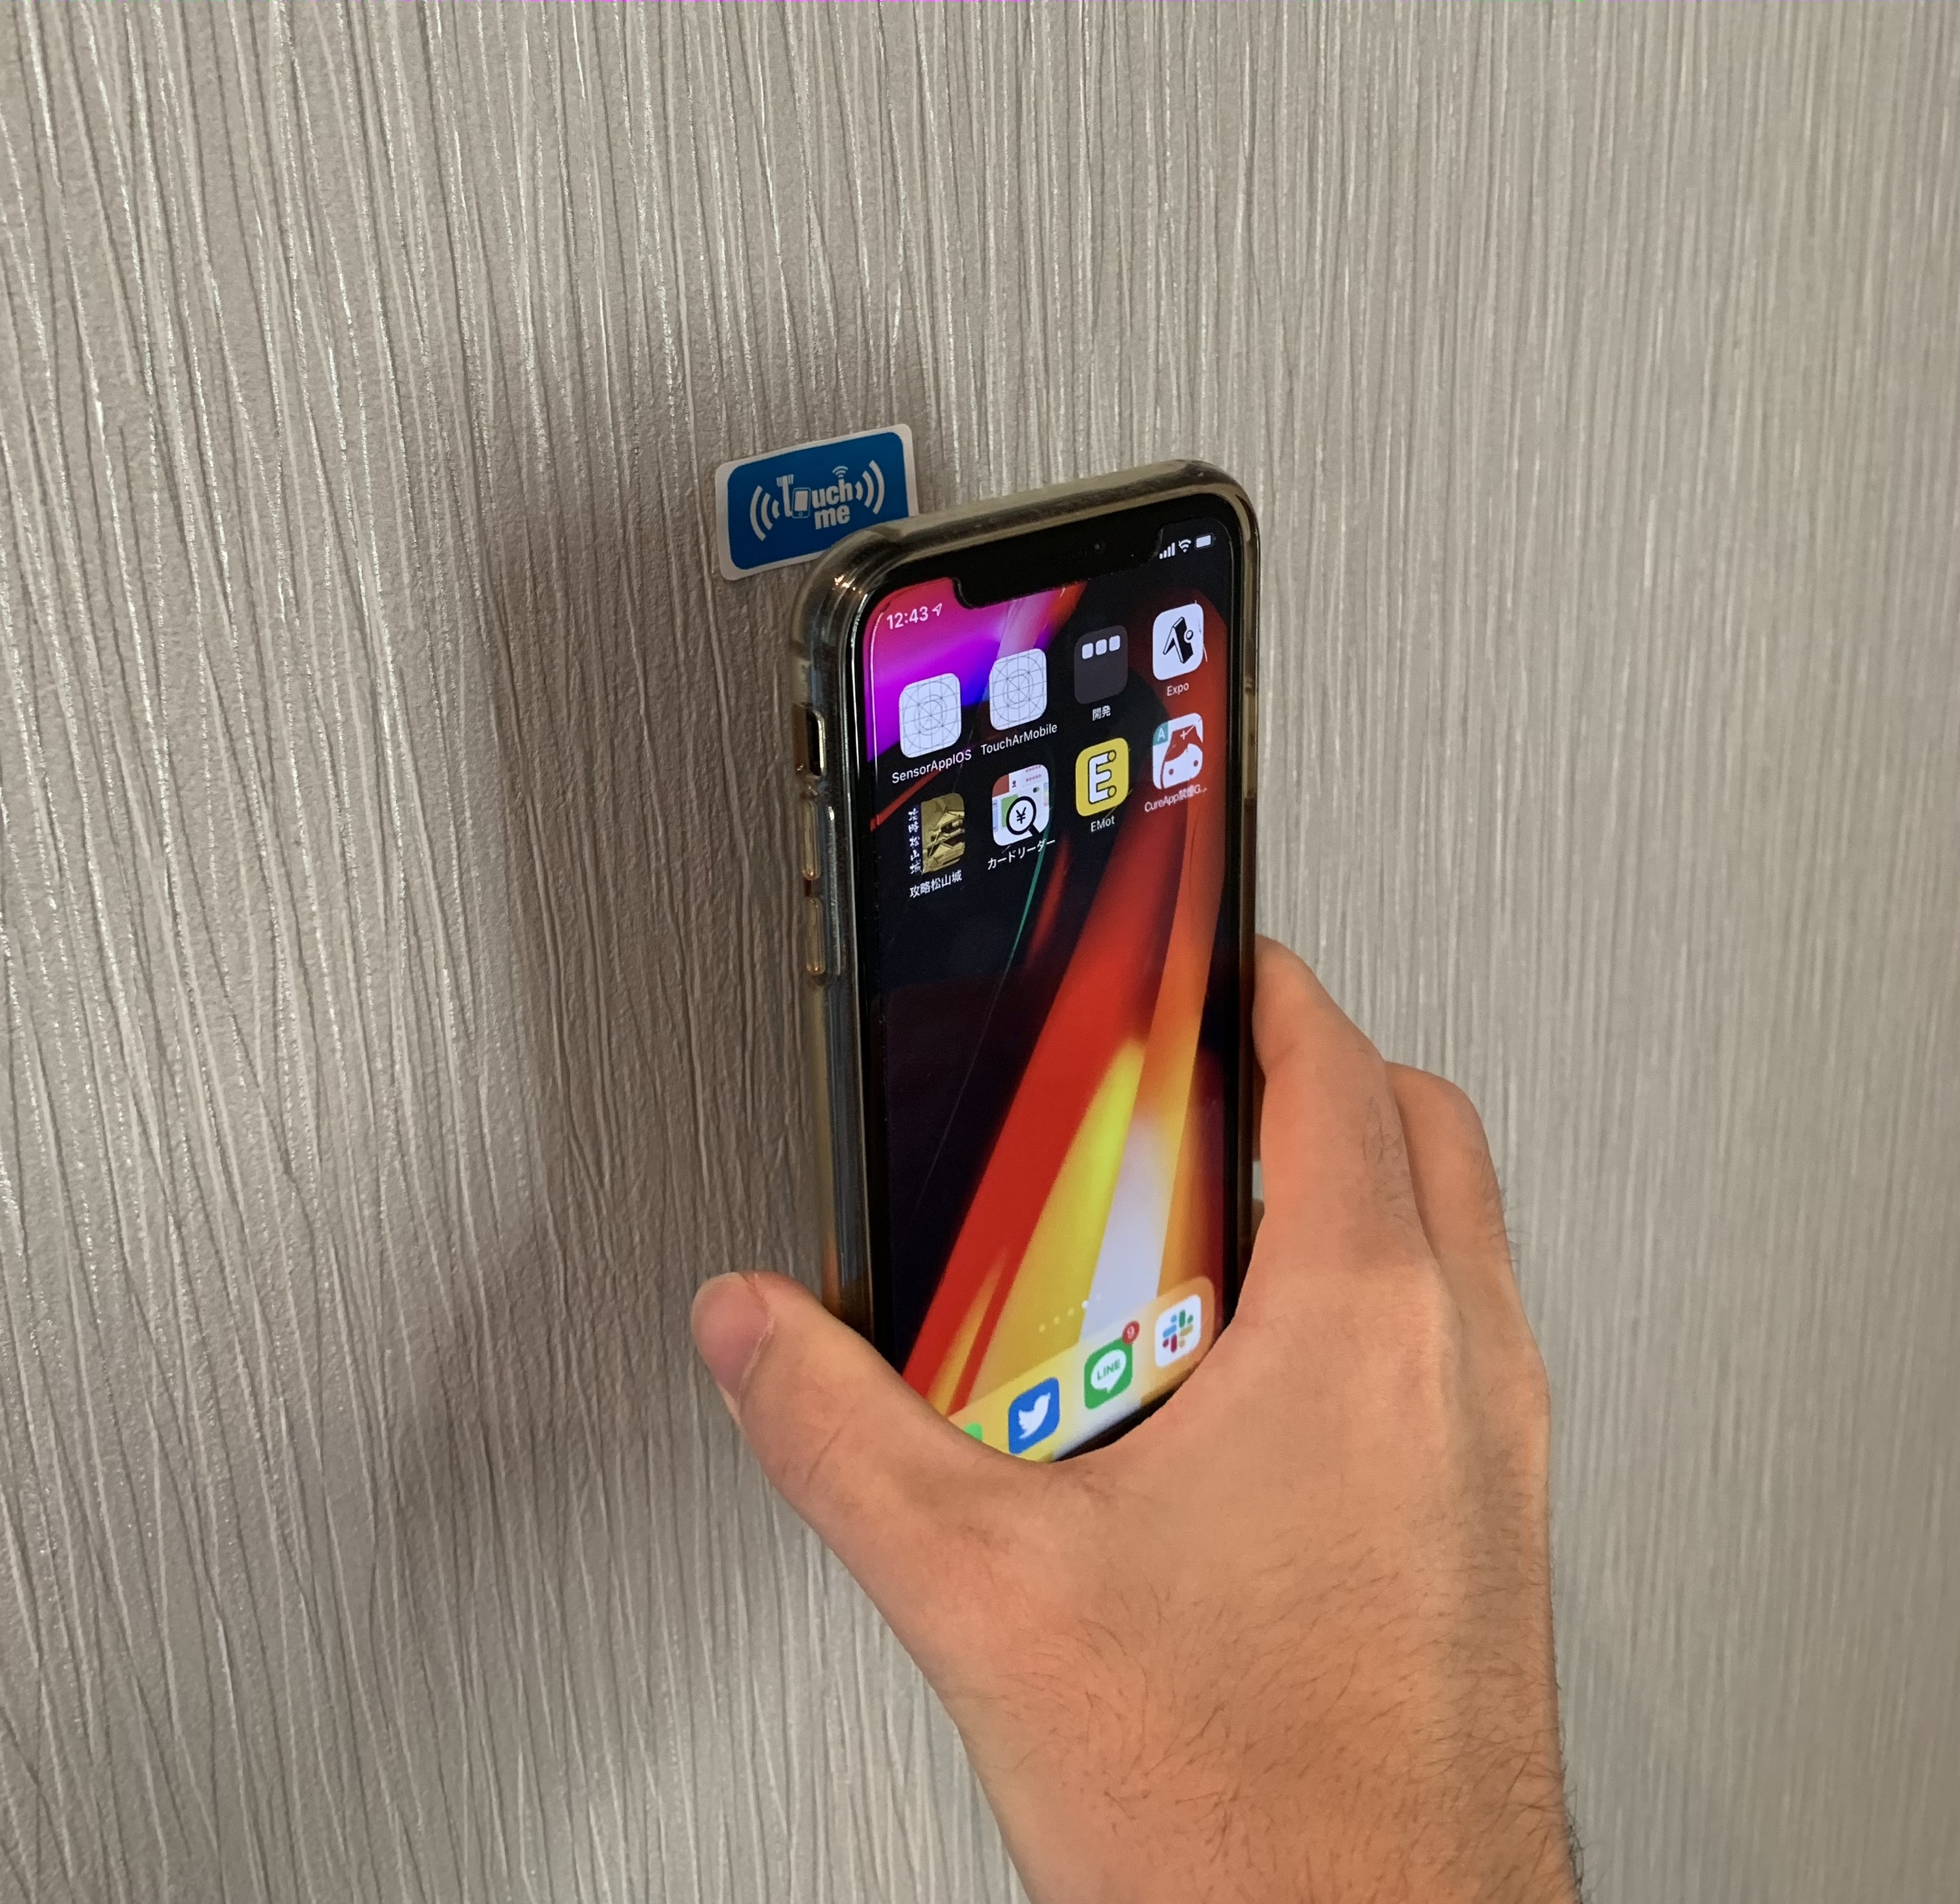
\includegraphics[width=100mm]{images/touch_nfc.jpg}
  \caption{NFCタグにタッチする様子} \label{fig:touch_nfc}
\end{figure}

\begin{figure}[h]
  \begin{minipage}{0.5\hsize}
    \centering
    \includegraphics[width=70mm]{images/hypar_touch_init_screen.png}
    \caption{ARでの表示} \label{fig:hypar_touch_init_screen}
  \end{minipage}
  \begin{minipage}{0.5\hsize}
    \centering
    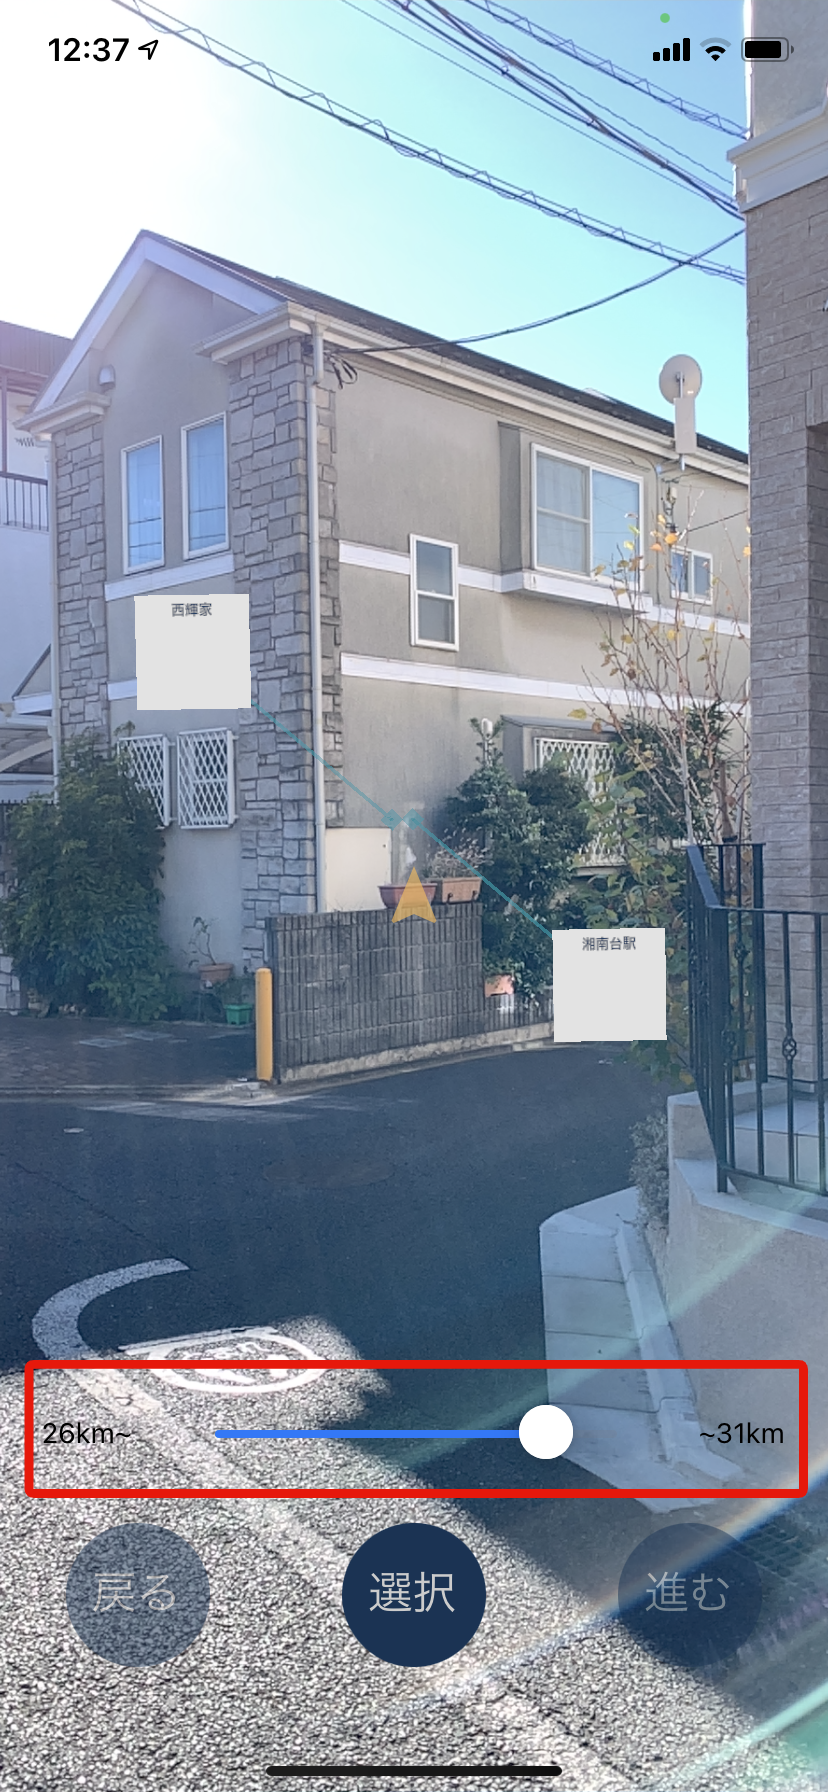
\includegraphics[width=70mm]{images/hypar_touch_slider.png}
    \caption{スライダーによる距離指定} \label{fig:hypar_touch_slider}
  \end{minipage}
\end{figure}

\paragraph*{表示されたAR情報の関連情報を表示・選択する}
画面の中央には三角のカーソルが表示されており、これをAR表示された情報の上に重ねると青く縁取られる様になっている。(図\ref{fig:hypar_touch_hover})
その状態で画面下部の選択ボタンを押すと図\ref{fig:hypar_touch_selected}のように関連する情報が放射状に表示される。
これらの放射状に表示された情報も同じようにカーソルで選択することができる。(\ref{fig:hypar_touch_sub_selected})
このように関連情報を選択していくことによって興味のある情報をAR上で探索することができる。

\begin{figure}[h]
  \begin{minipage}{0.5\hsize}
    \centering
    \includegraphics[width=70mm]{images/hypar_touch_hover.png}
    \caption{カーソルを重ねた状態} \label{fig:hypar_touch_hover}
  \end{minipage}
  \begin{minipage}{0.5\hsize}
    \centering
    \includegraphics[width=70mm]{images/hypar_touch_selected.png}
    \caption{選択した状態} \label{fig:hypar_touch_selected}
  \end{minipage}
\end{figure}

\begin{figure}[h]
    \centering
    \includegraphics[width=70mm]{images/hypar_touch_sub_selected.png}
    \caption{関連情報の選択} \label{fig:hypar_touch_sub_selected}
\end{figure}

\paragraph*{選択されたAR情報の詳細を見る}
上記のようにカーソルをAR情報にあわせた上で選択ボタンを押すと上部には図\ref{fig:hypar_touch_top}のように選択された情報のタイトルの他に「see more」と書かれたボタンが出現する。
これをクリックすることでAR情報の元となったScrapboxをみることが可能である。(図\ref{fig:hypar_touch_webview})

\begin{figure}[h]
  \begin{minipage}{0.5\hsize}
    \centering
    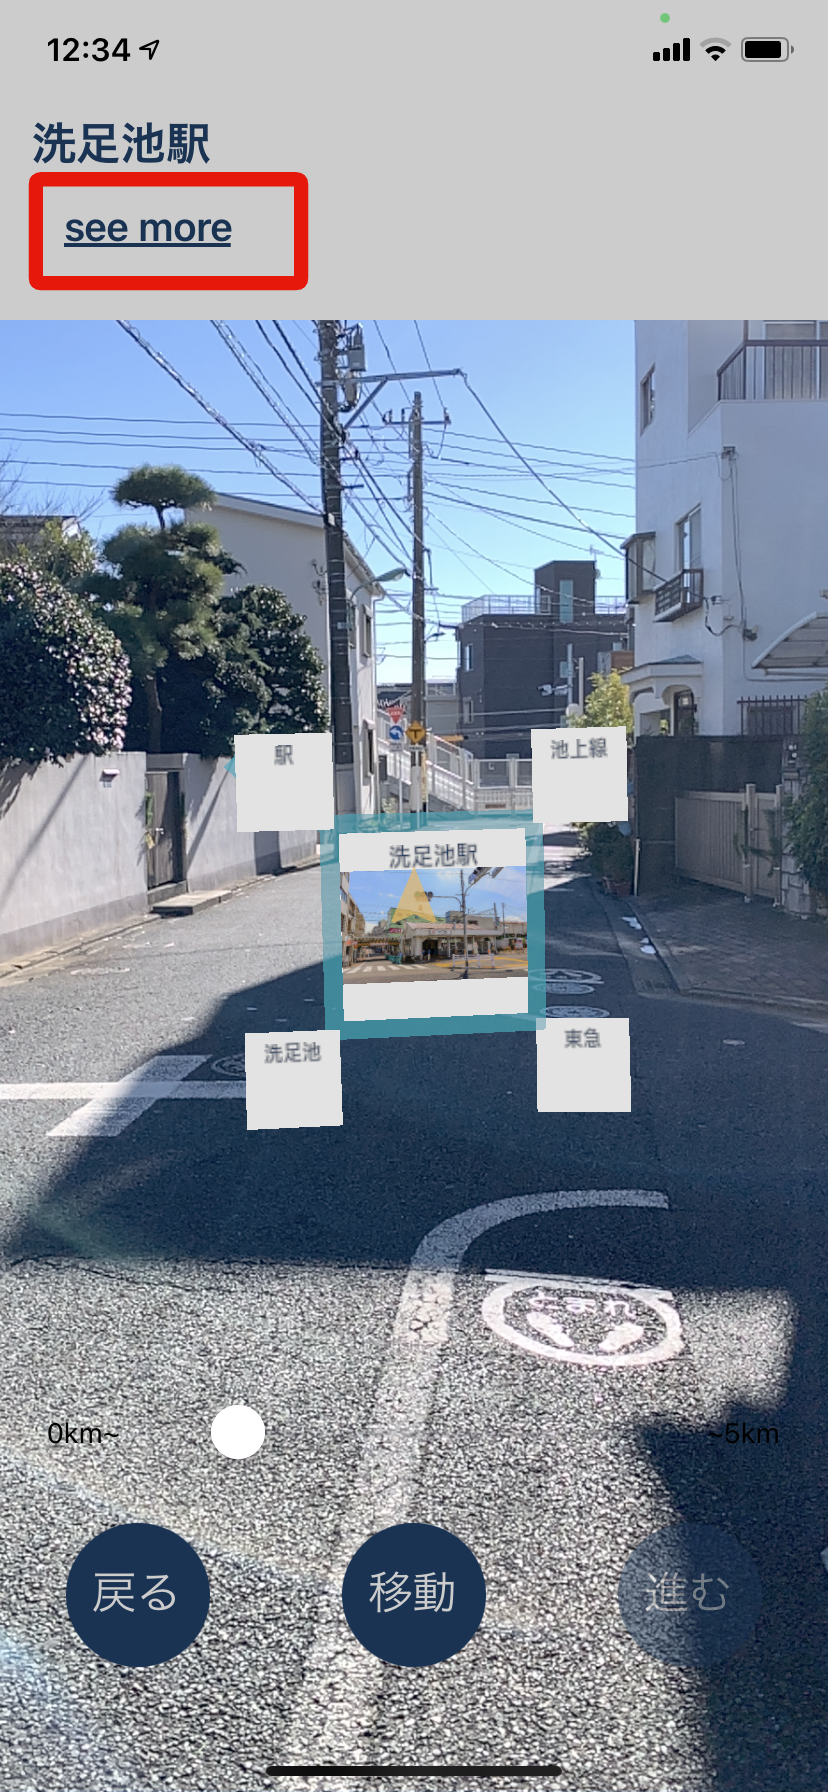
\includegraphics[width=70mm]{images/hypar_touch_top.png}
    \caption{詳細を表示するボタン} \label{fig:hypar_touch_top}
  \end{minipage}
  \begin{minipage}{0.5\hsize}
    \centering
    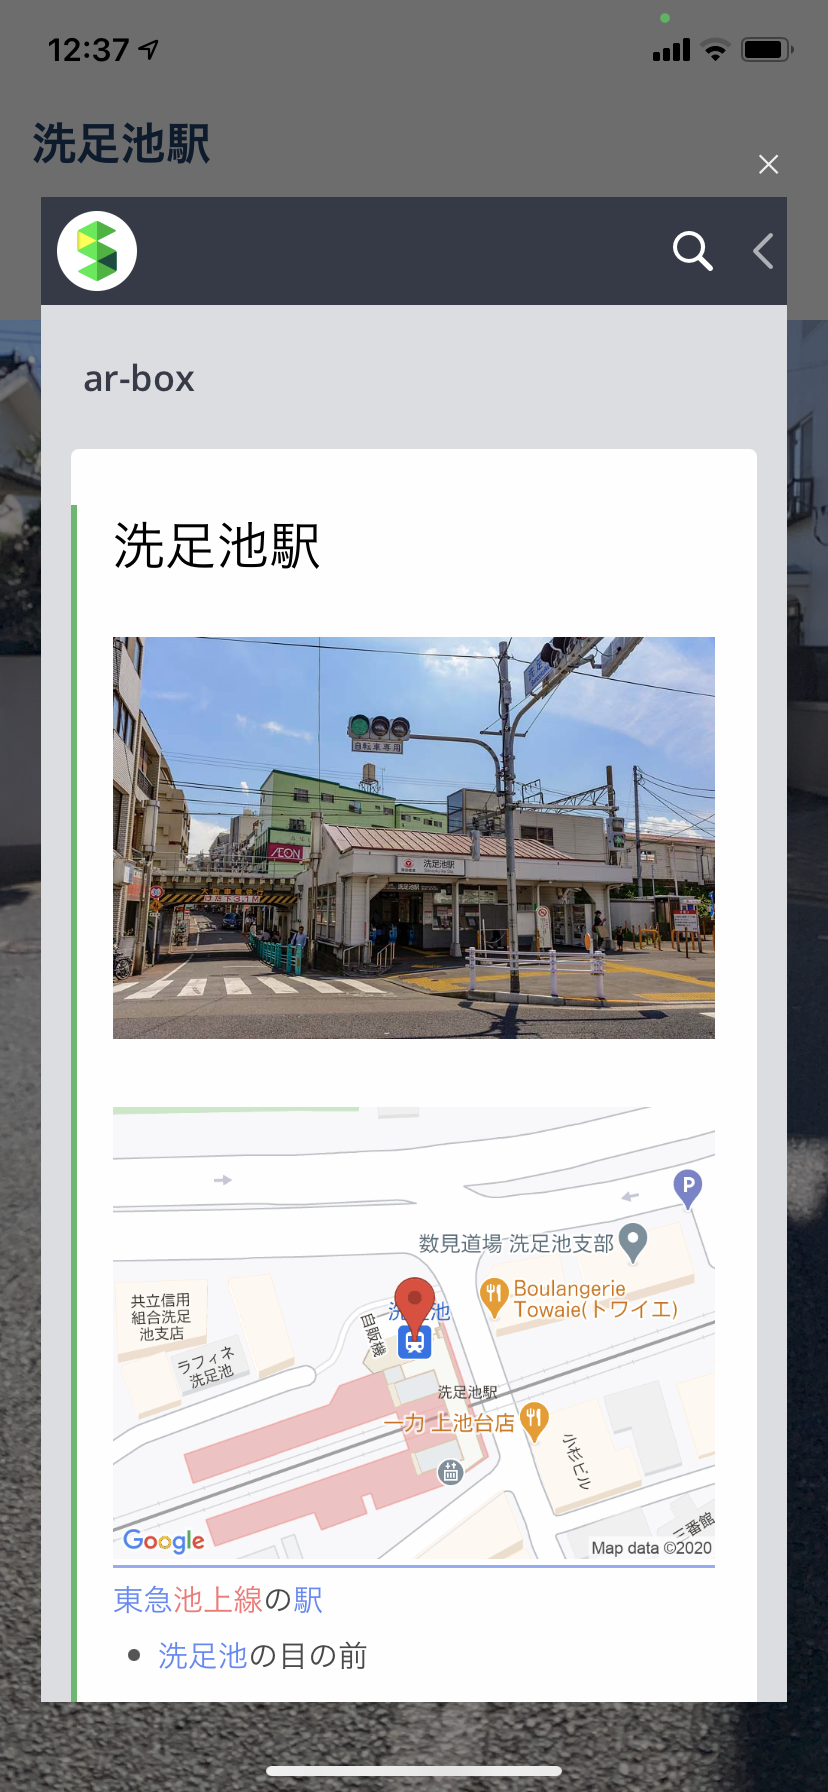
\includegraphics[width=70mm]{images/hypar_touch_webview.png}
    \caption{Scrapboxでの情報表示} \label{fig:hypar_touch_webview}
  \end{minipage}
\end{figure}

\paragraph*{選択されたAR情報の場所に視点を移動する}
同じようにカーソルをAR情報にあわせた上で選択ボタンを押し、もう一度選択したAR情報にカーソルを持っていくと下部中央のボタンが「移動」に変化する(図\ref{fig:hypar_touch_move_button})
この移動ボタンを押すと図\ref{fig:hypar_touch_move_map}mapでの移動アニメーションを経て選択された AR情報がある場所からのビュー(図\ref{fig:hypar_touch_moved})に切り替えることができる。

\begin{figure}[h]
  \begin{minipage}{0.5\hsize}
    \centering
    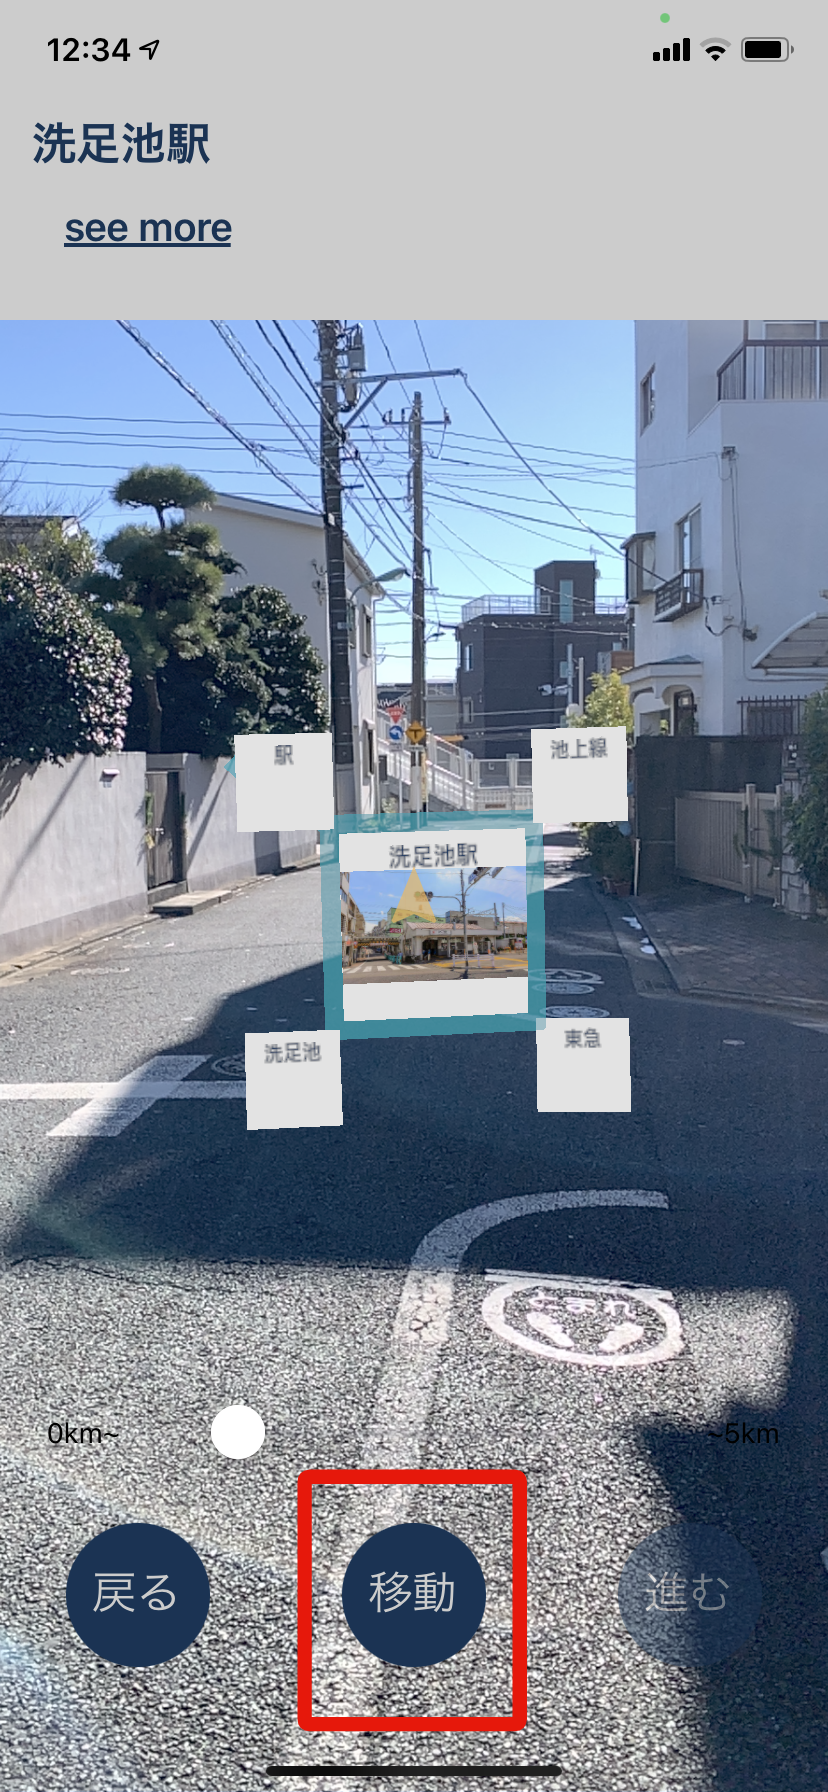
\includegraphics[width=70mm]{images/hypar_touch_move_button.png}
    \caption{移動ボタン} \label{fig:hypar_touch_move_button}
  \end{minipage}
  \begin{minipage}{0.5\hsize}
    \centering
    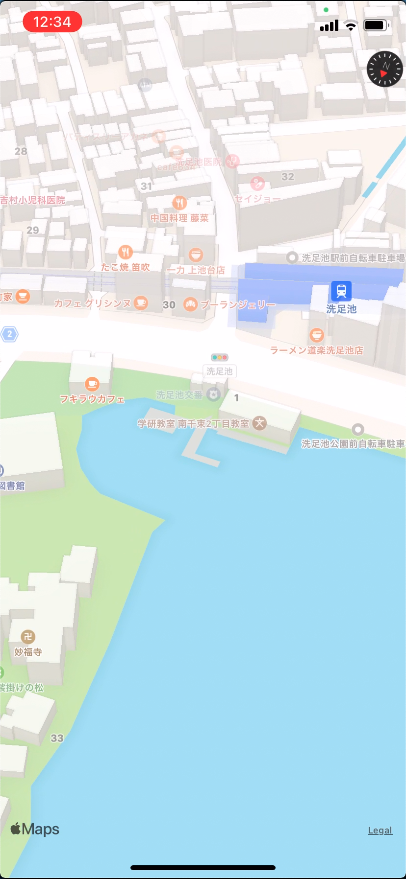
\includegraphics[width=70mm]{images/hypar_touch_move_map.png}
    \caption{Mapでの移動アニメーション} \label{fig:hypar_touch_move_map}
  \end{minipage}
\end{figure}

\begin{figure}[h]
  \centering
  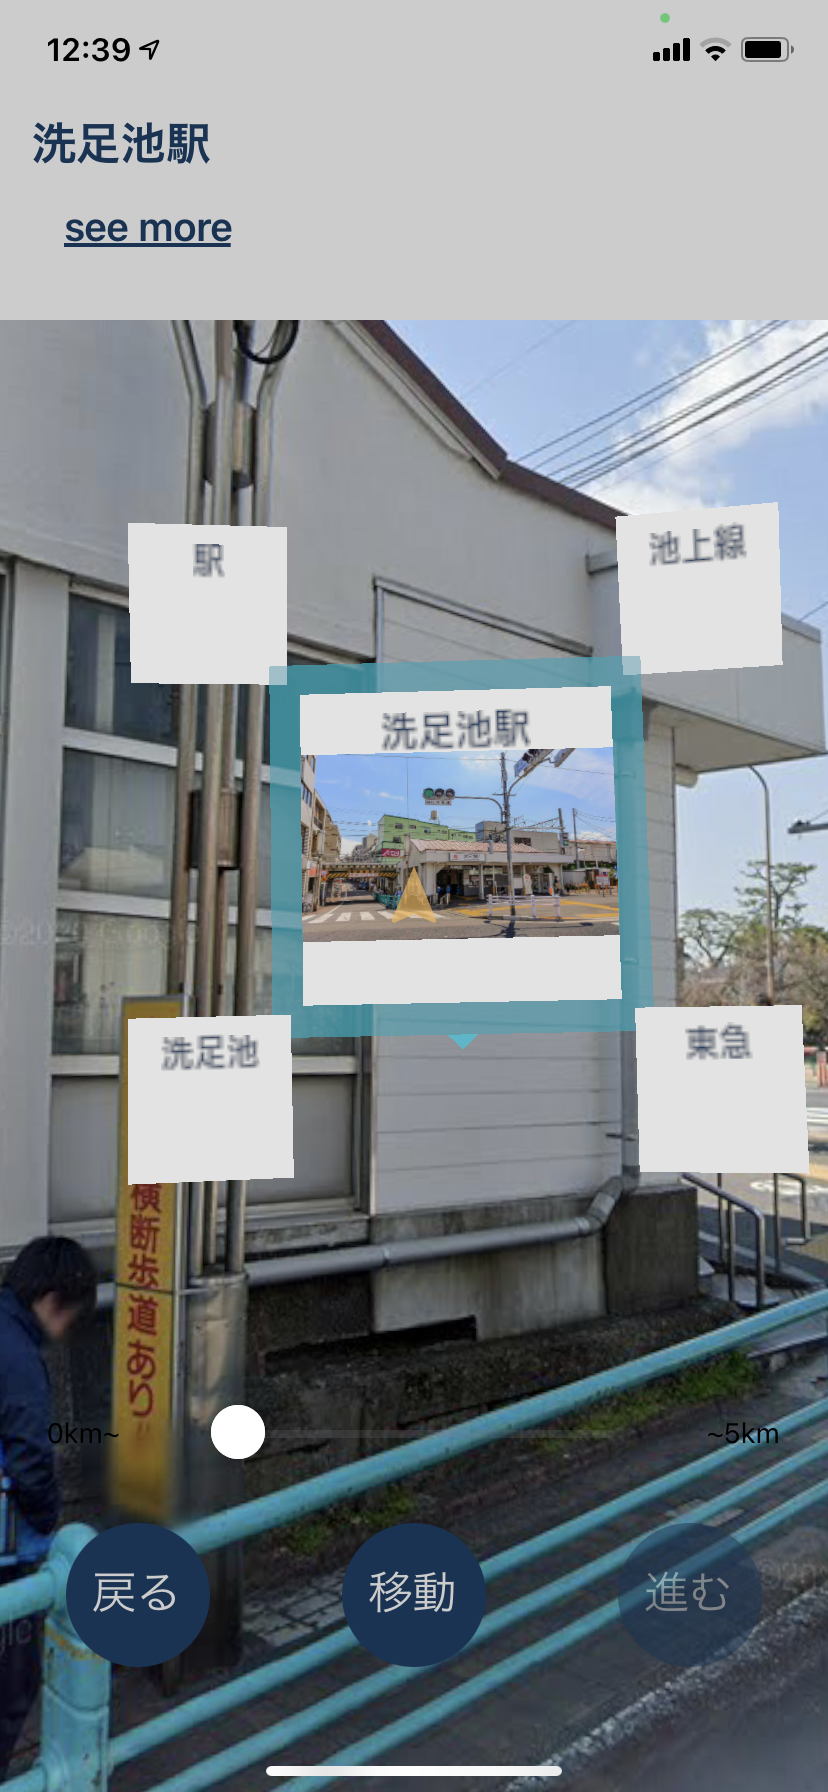
\includegraphics[width=70mm]{images/hypar_touch_moved.png}
  \caption{移動先での表示} \label{fig:hypar_touch_moved}
\end{figure}

\paragraph*{AR情報の選択を解除する・前の状態に戻る}
上記のような選択状態はAR情報のない画面をタップすることで解除できる。
また選択や移動した履歴情報を常に保存しており、画面下部の「戻る」「進む」ボタン(図\ref{fig:hypar_touch_history_button})で戻ったり進んだりすることができる。

\begin{figure}[h]
  \centering
  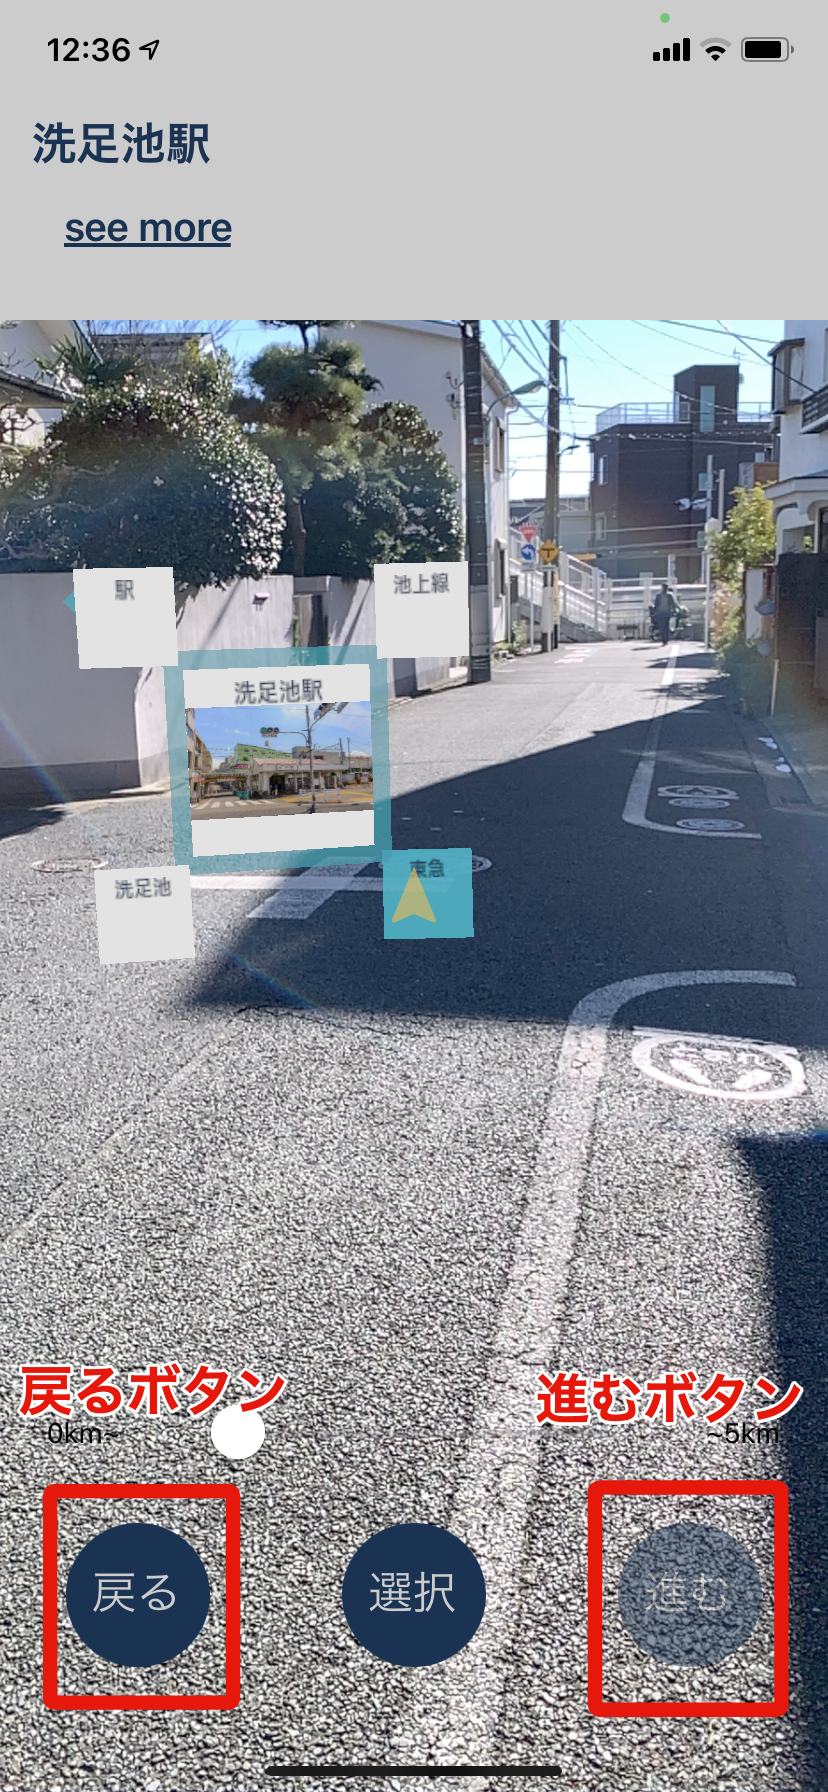
\includegraphics[width=70mm]{images/hypar_touch_history_button.png}
  \caption{進むボタンと戻るボタン} \label{fig:hypar_touch_history_button}
\end{figure}

\subsubsection{ScrapboxによるAR情報法の追加・編集}
HypAR Touchアプリに表示されるAR情報はNFCタグ指定されたScrapboxのプロジェクトをもとに生成されている。
Scrapboxのプロジェクトにあるページのうち、Location記法によって地理情報の記述のあるページがアプリ側で表示されるAR情報と対応する。

\paragraph*{ARで表示する情報を追加する}
AR情報はScrapboxのページと対応しているため、新しくページを作成し、以下の2点の情報を記入することでAR情報が登録される。
\begin{itemize}
  \item ページタイトル
  
  図\ref{fig:scrapbox_ar_new}の\textcircled{\scriptsize{1}}部分であり、ページを作る上で必須となる。
  タイトルはAR表示でサムネイルのの上に表示されるものと対応する。

  \item Location記法による記述
  
  Scrapboxにはソースコード \ref{google_map_url}のようなGoogle MapsのURLをソースコード \ref{location}のようなLocation記法に変換し、図\ref{fig:scrapbox_ar_new}の\textcircled{\scriptsize{2}}のようにマップとして表示する機能がある。
  この機能を利用し利用しARの情報を追加したい場所を中心にしたGoogle MapsのURLをScrapboxに貼り付けることでARの情報登録できる。

  \begin{lstlisting}[caption=googleMapのURL, label=google_map_url]
    https://www.google.com/maps/place/%E6%9D%B1%E4%BA%AC%E9%A7%85/@35.681502,139.7671784,17z/data=!4m5!3m4!1s0x60188bfbd89f700b:0x277c49ba34ed38!8m2!3d35.6812362!4d139.7671248
  \end{lstlisting}

  \begin{lstlisting}[caption=Location記法, label=location]
    [N35.681502,E139.7671784,Z16 東京駅]
  \end{lstlisting}
\end{itemize}

\begin{figure}[h]
  \centering
  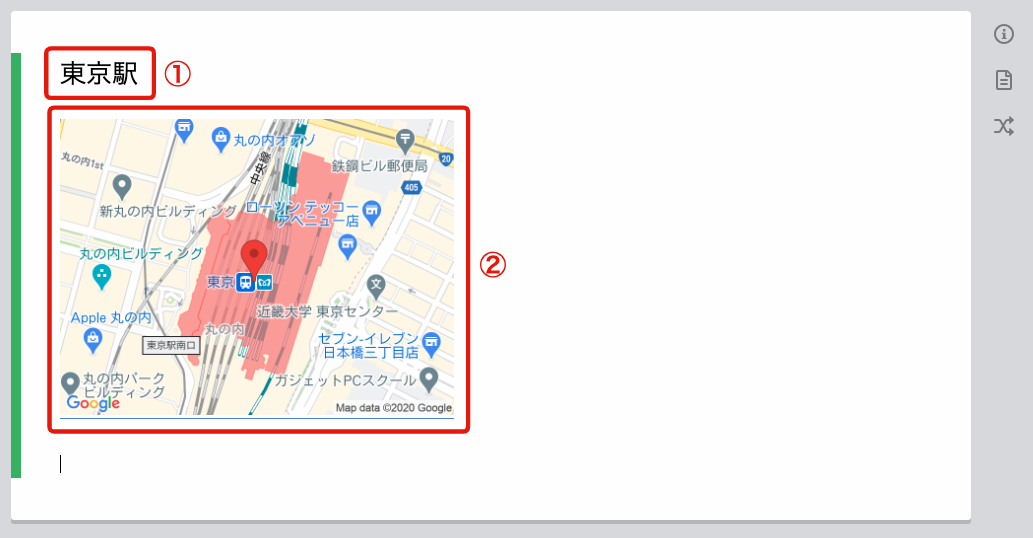
\includegraphics[width=120mm]{images/scrapbox_ar_new.png}
  \caption{新しくページを作成した時} \label{fig:scrapbox_ar_new}
\end{figure}

\paragraph*{サムネイルを追加する}
Scrapboxでは画像のURLを\texttt{[]}で囲う、または画像をドラッグ・アンド・ドロップすることで図\ref{fig:scrapbox_thumbnail}のようにページに画像を表示させることができる。
このようにScrapboxのページに画像を貼ると、一番上にある画像がAR表示でのサムネイルになる。(図\ref{fig:scrapbox_thumbnail_and_ar})

\begin{figure}[h]
  \centering
  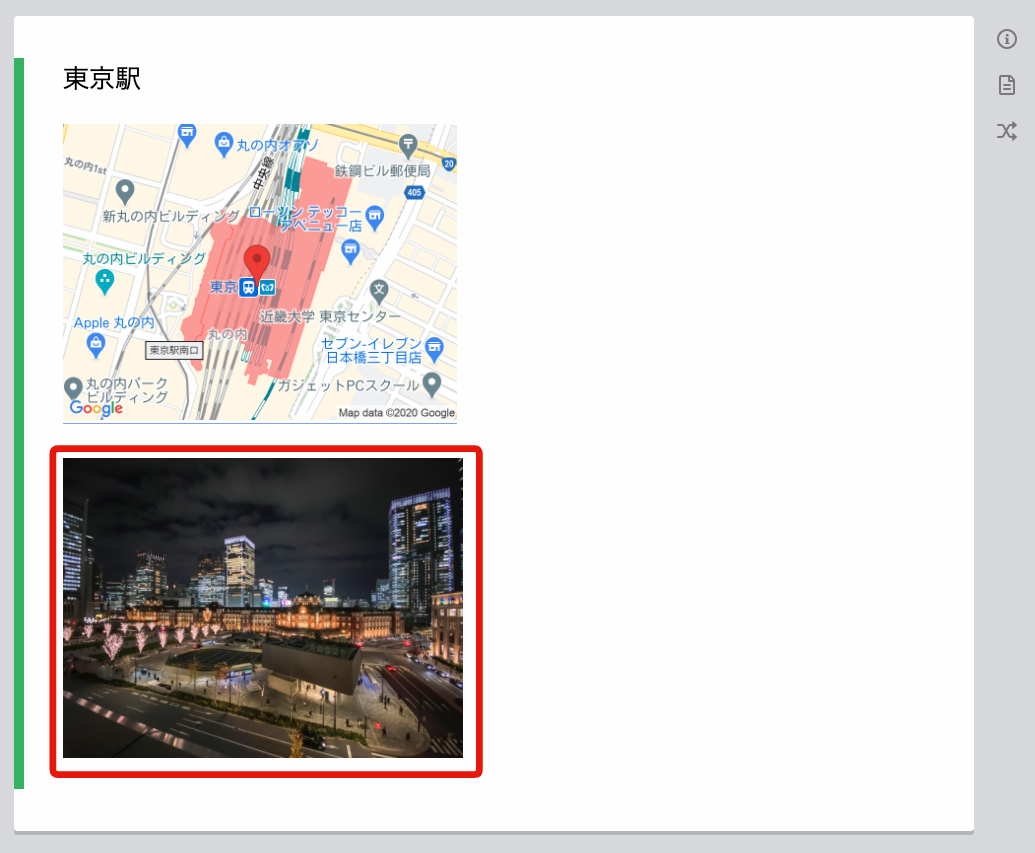
\includegraphics[width=120mm]{images/scrapbox_thumbnail.png}
  \caption{Scrapboxに貼り付けた画像} \label{fig:scrapbox_thumbnail}
\end{figure}

\begin{figure}[h]
  \centering
  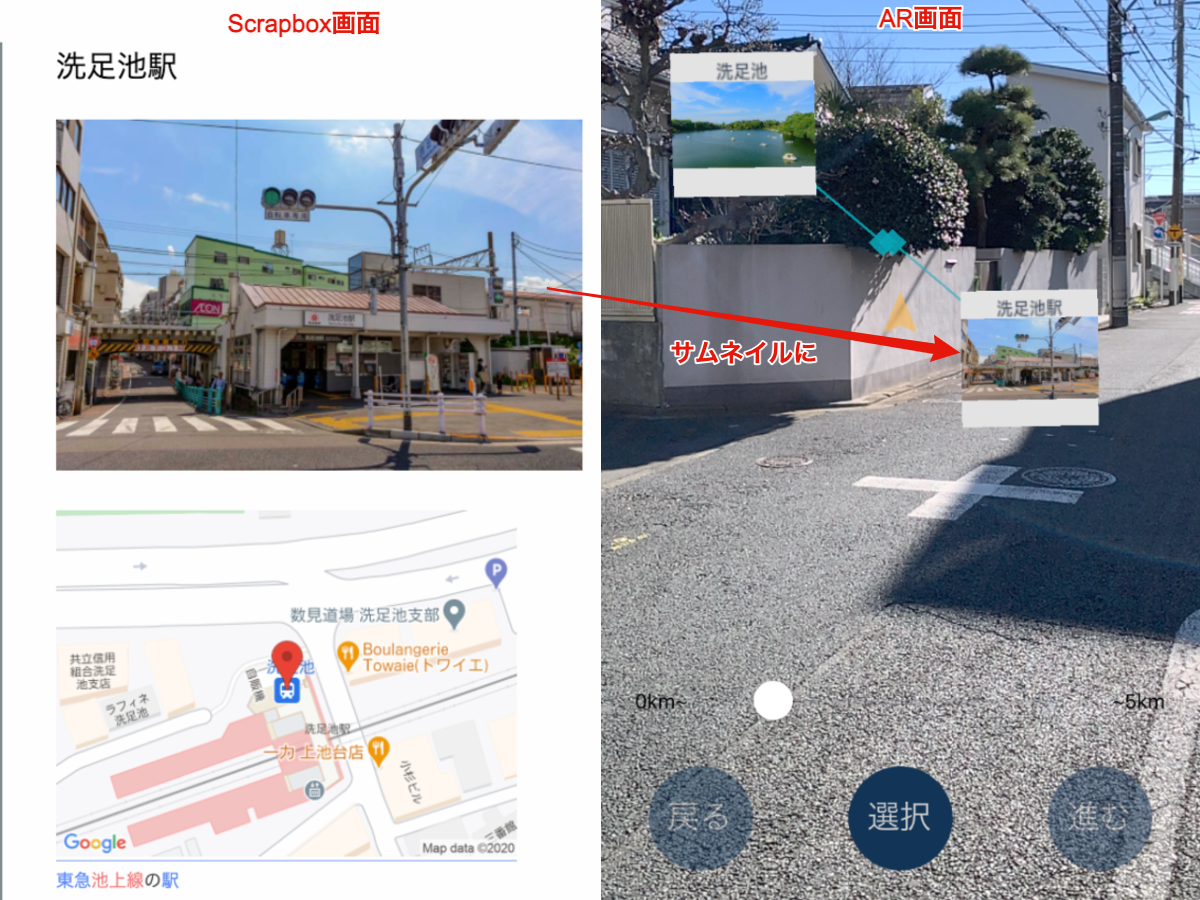
\includegraphics[width=120mm]{images/scrapbox_thumbnail_and_ar.png}
  \caption{Scrapbox上の画像とARでの表示} \label{fig:scrapbox_thumbnail_and_ar}
\end{figure}

\paragraph*{ハイパーリンクを利用して説明を書く}
Scrapboxでは単語を\texttt{[]}で囲うことにより同一wiki内ページへのハイパーリンクを含んだ文章を記述することが可能である。
他ページヘのハイパーリンクが生成されるとAR表示で関連情報として表示されるようになる。(図\ref{fig:scrapbox_link_and_ar})
説明に利用した単語を積極的にリンクにすることによって関連する情報を提示することが可能になる。

\begin{figure}[h]
  \centering
  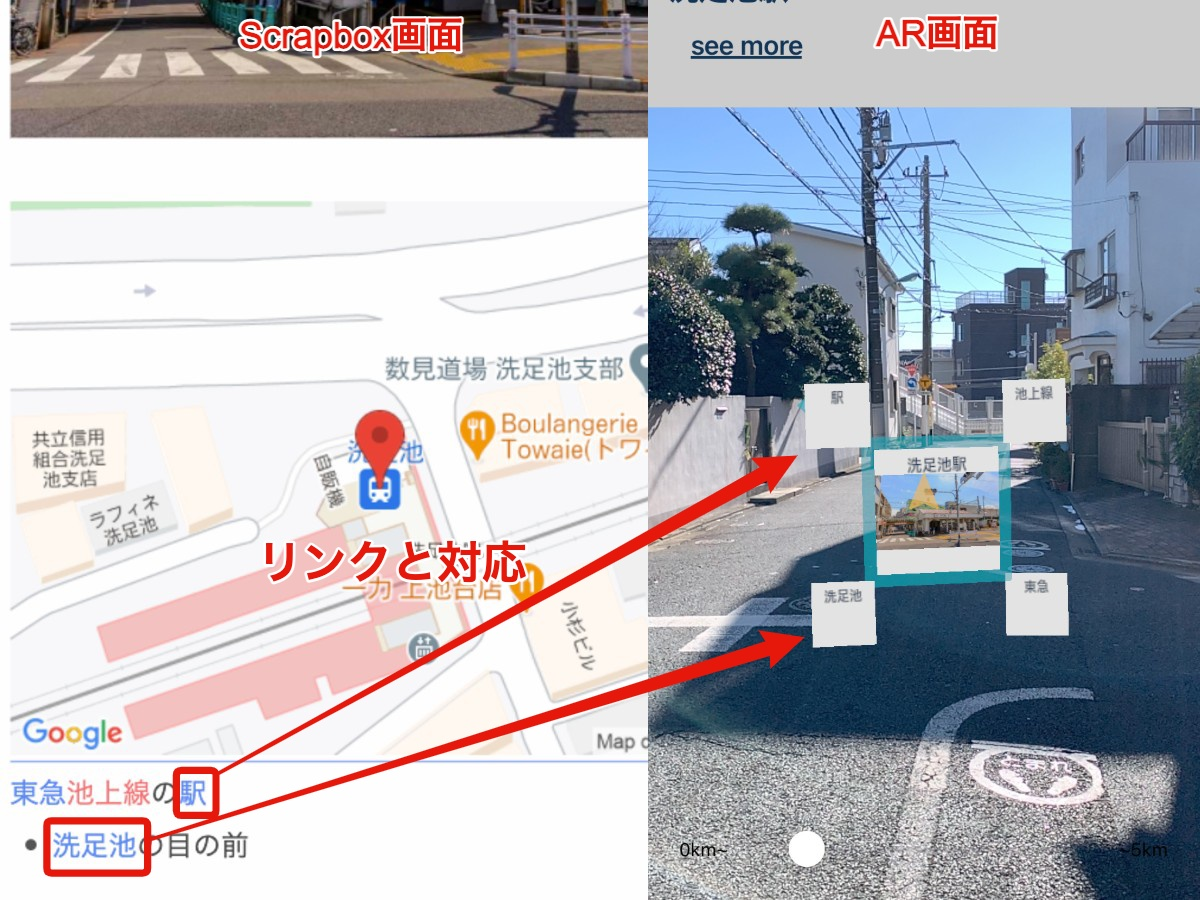
\includegraphics[width=120mm]{images/scrapbox_link_and_ar.jpg}
  \caption{Scrapbox上のリンクとARでの表示} \label{fig:scrapbox_link_and_ar}
\end{figure}

\subsubsection{NFCタグに対する情報の書き込み}
NFCタグにはISO/IEC 14443 TypeAに準拠したNTAGを利用する。
NFCに記録するNFCで情報を記録する際に一般的なNDEFフォーマットで情報を書き込む。
書き込む情報は図\ref{fig:nfc_uri}のようにCustomURLSchemeに沿ったURIの形式で書き込む。

\begin{figure}[h]
  \centering
  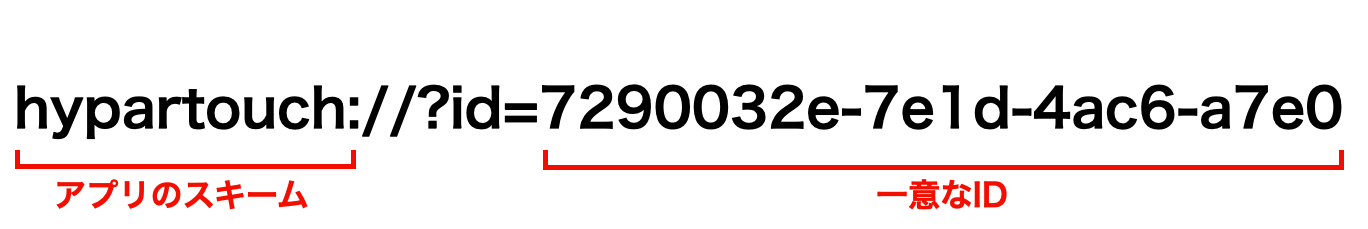
\includegraphics[width=120mm]{images/nfc_uri.png}
  \caption{NFCに書き込むURIデータ} \label{fig:nfc_uri}
\end{figure}

その上でタグに書き込んだIDと紐付ける形でHypAR Touchのサーバーに以下の情報を登録する。
\begin{itemize}
  \item 緯度経度
  \item タグの設置される向き(0〜360度)
  \item 表示するAR情報の元となるScrapboxのプロジェクト
  \item タッチした時に選択されているリンク情報
\end{itemize}
これらの情報はHypAR Touchアプリ内の登録画面(図\ref{fig:nfc_register_mobile})により登録可能である。

\begin{figure}[h]
  \centering
  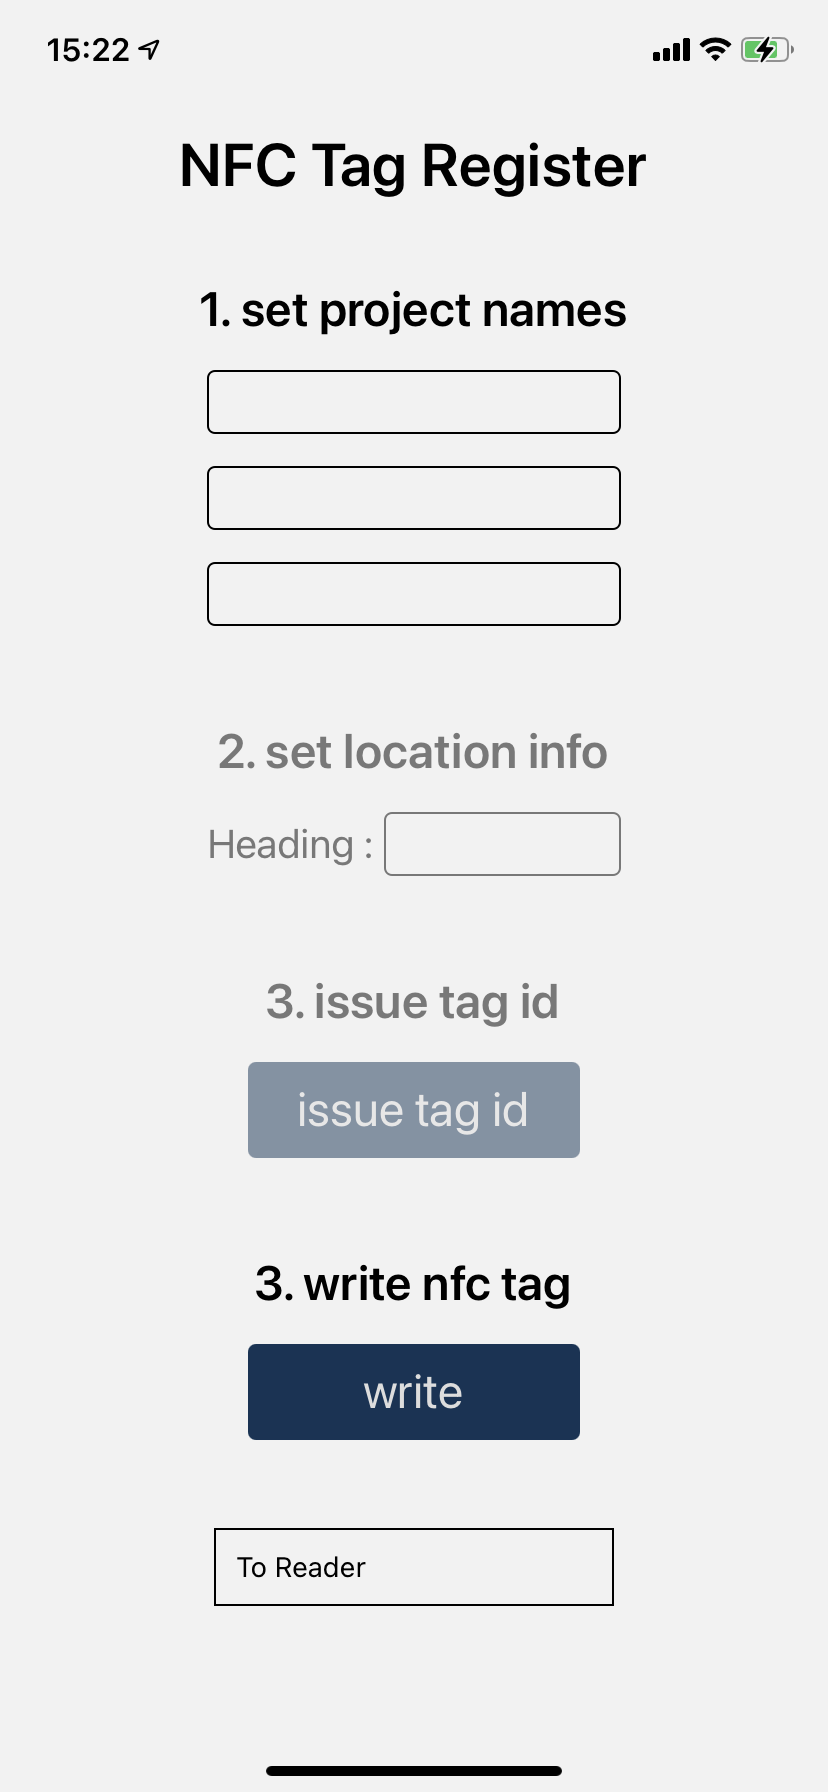
\includegraphics[width=70mm]{images/nfc_register_mobile.png}
  \caption{モバイルアプリでの登録} \label{fig:nfc_register_mobile}
\end{figure}